\documentclass[tikz,border=3pt]{standalone}
\usepackage[utf8]{inputenc}
\usepackage[T1]{fontenc}
\usepackage{lmodern}
\renewcommand{\familydefault}{\sfdefault}
\usepackage{sansmath}\sansmath
\usepackage{chemfig}
\usepackage{pgfplots}\pgfplotsset{compat=1.18,/pgf/number format/use comma,/pgf/number format/1000 sep={.}}
\usetikzlibrary{arrows.meta,calc,positioning,decorations.pathmorphing,patterns}
% paleta del sitio
\definecolor{nar}{HTML}{E8680C}\definecolor{narc}{HTML}{FFB35C}\definecolor{hielo}{HTML}{FFF3E8}
\definecolor{tinta}{HTML}{1D1D1F}\definecolor{gris}{HTML}{6E6E73}\definecolor{lila}{HTML}{7C5CF0}
\definecolor{azul}{HTML}{2F6FD6}\definecolor{menta}{HTML}{17A673}\definecolor{coral}{HTML}{E8342A}
\begin{document}
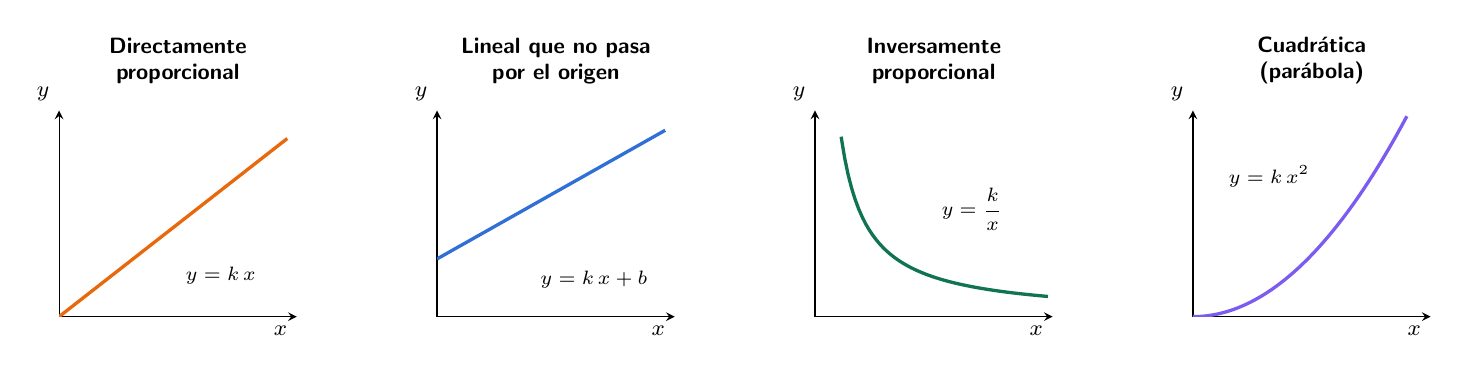
\begin{tikzpicture}[font=\footnotesize]
\pgfplotsset{mini/.style={width=4.6cm,height=4.2cm,axis lines=left,xmin=0,xmax=5,ymin=0,ymax=5,ticks=none,xlabel={$x$},ylabel={$y$},xlabel style={at={(1,0)},anchor=north east},ylabel style={rotate=-90,at={(0,1)},anchor=south east},title style={font=\footnotesize\bfseries,align=center},every axis plot/.append style={very thick,samples=60}}}
\begin{axis}[mini,title={Directamente\\proporcional}]
\addplot[nar,domain=0:4.8] {0.9*x};
\node[font=\scriptsize] at (axis cs:3.4,1.0) {$y = k\,x$};
\end{axis}
\begin{axis}[mini,xshift=4.8cm,title={Lineal que no pasa\\por el origen}]
\addplot[azul,domain=0:4.8] {1.4+0.65*x};
\node[font=\scriptsize] at (axis cs:3.3,0.9) {$y = k\,x + b$};
\end{axis}
\begin{axis}[mini,xshift=9.6cm,title={Inversamente\\proporcional}]
\addplot[menta!70!black,domain=0.55:4.9] {2.4/x};
\node[font=\scriptsize] at (axis cs:3.3,2.6) {$y = \displaystyle\frac{k}{x}$};
%\rac{k}{x}$};
\end{axis}
\begin{axis}[mini,xshift=14.4cm,title={Cuadrática\\(parábola)}]
\addplot[lila,domain=0:4.5] {0.24*x^2};
\node[font=\scriptsize] at (axis cs:1.6,3.4) {$y = k\,x^2$};
\end{axis}
\end{tikzpicture}
\end{document}
